\documentclass{beamer}

\mode<presentation>
{
  \usetheme{CambridgeUS}
  % \setbeamercovered{transparent}
}

\usepackage[T1]{fontenc}
\usepackage[utf8]{inputenc}
\usepackage[spanish]{babel}
\usepackage{color}
\usepackage{hyperref}
\usepackage{algorithm,algorithmic}
\usepackage{colortbl}
\usepackage{graphicx}
\usepackage{multicol}
\usepackage{enumitem}
\setitemize{itemsep=1.2em,%
  label=\usebeamerfont*{itemize item}%
  \usebeamercolor[fg]{itemize item}%
  \usebeamertemplate{itemize item}
}

\usepackage{minted}
\usepackage[skins,minted]{tcolorbox}

\newcommand{\code}[1]{\mintinline{java}{#1}}
\newcommand{\codet}[1]{\texttt{#1}}

\setminted[java]{
  linenos=true,
  fontfamily=tt,
  fontsize=\small,
  frame=leftline,
  autogobble=True,
}

\newminted[jsmall]{java}{
  fontsize=\footnotesize
  , linenos = false
  , frame=single
  , autogobble=true
}

\newtcblisting{java}[2][]{
  minted language=java,
  enhanced, listing engine=minted,
  listing only, #1, title=#2, left=2em
}

\setminted[bash]{
  linenos=true,
  fontfamily=tt,
  fontsize=\small,
  frame=leftline
}

\newtcblisting{bash}[2][]{minted language=bash,
  enhanced, listing engine=minted,
  listing only, #1, title=#2, left=2em
}

\title[\textbf{Programación 2}]{\textbf{Programación 2}}
\subtitle{Java Collections Framework}

\author[IF-EG]
{Profesores:\\
  Ismael Figueroa -  \texttt{\small ifigueroap@gmail.com} \\
  \vspace{0.5mm}
  Eduardo Godoy - \texttt{\small eduardo.gl@gmail.com}
}

\institute[Universidad de Valparaíso]

\date{}

\begin{document}

\begin{frame}
  \titlepage
\end{frame}

% https://docs.oracle.com/javase/tutorial/collections/

\section{¿Qué es una Collection?}

\begin{frame}
  \frametitle{¿Qué es una Collection ?}

  \begin{block}{Definición}
    Una \emph{Collection} es simplemente \textbf{\textit{un objeto que
        agrupa múltiples objetos en una sola unidad}}.
  \end{block}
    
  \begin{itemize}

  \item Se usan para \textbf{almacenar}, \textbf{manipular}, y
    \textbf{comunicar} datos agregados.
     
  \item Representan datos asociados de forma natural en el dominio del
    problema: una mano de cartas, un listado teléfonico, etc.
    
  \item Ya hemos usado una collection: \codet{List} y \codet{ArrayList}!
    
  \end{itemize}
  
\end{frame}


\begin{frame}
  \frametitle{¿Qué es el Java Collections Framework?}

  Es una \textbf{arquitectura unificada} para representar y manipular
  collections, que consiste
  de:\footnote{\url{https://docs.oracle.com/javase/tutorial/collections/intro/index.html}}

  \begin{small}

  \begin{itemize}
  \item \textbf{Interfaces}: son representaciones abstractas de las
    colecciones. Permiten la manipulación de colecciones sin importar
    su implementación actual, explotando los mecanismos de
    polimorfismo.
    
  \item \textbf{Implementaciones}: son implementaciones concretas de
    las colecciones, que implementan las interfaces. Sirven como
    código general y reutilizable que podemos aprovechar en todos
    nuestros programas.
    
  \item \textbf{Algoritmos}: son métodos para realizar operaciones
    útiles con las colecciones: buscar, ordenar, etc. Los algoritmos
    también aprovechan el polimorfismo para realizar \emph{operaciones
      genéricas}.
    
  \end{itemize}
  \end{small}
  
\end{frame}

\begin{frame}
  \frametitle{¿Qué beneficios tiene el Java Collections Framework?}

  \begin{itemize}
    
  \item \textbf{Reducir el esfuerzo de programación:} al usar
    colecciones pre-existentes podemos enfocarnos en las operaciones
    \emph{interesantes y relevantes} de nuestro programa, más que en
    los detalles de cómo almacenar y obtener los datos.
    
  \item \textbf{Aumentar la velocidad y calidad de programación:} las
    implementaciones estándar son de alta calidad y performance. En
    caso de necesidad pueden ser cambiadas sin alterar el resto de los
    programas.
    
  \end{itemize}
  
\end{frame}

\begin{frame}
  \frametitle{¿Qué beneficios tiene el Java Collections Framework?}

  \begin{itemize}
    
  \item \textbf{Permite interoperabilidad entre programas:} distintas
    aplicaciones, incluso desarrolladas de manera independiente,
    pueden \emph{intercambiar datos de manera transparente} mediante
    el paso de colecciones como parámetros.
    
  \item \textbf{Reduce el costo de aprendizajey diseño de APIs:} cada
    vez que desarrollamos un sistema, y sus respectivas interfaces
    públicas, podemos simplemente utilizar collecciones para manipular
    agregaciones de datos.
    
  \item \textbf{Fomenta la reutilización del software:} además de las
    implementaciones estándar, nuevas implementaciones se pueden
    agregar de manera transparente, siempre que cumplan con las
    interfaces requeridas.
    
  \end{itemize}
  
\end{frame}

\section{Las Interfaces}

\subsection{Interfaz \codet{java.util.Collection}}

\begin{frame}[fragile]
  \frametitle{Interfaz \codet{java.util.Collection}}

  La primera interfaz es
  \codet{java.util.Collection}\footnote{\url{https://docs.oracle.com/javase/8/docs/api/java/util/Collection.html}}.

\begin{minted}{java}
public interface Collection<E>
\end{minted}

  Esta interfaz define \textbf{la raíz de la jerarquía de interfaces
    de colecciones}. Define los métodos \textbf{obligatorios} que toda
  colección \textbf{debe} implementar. También define métodos
  \textbf{opcionales} que toda colección \textbf{puede} implementar.

  \begin{itemize}
  \item Los métodos opcionales son aquellos que indican \codet{throws
      UnsupportedOperationExpression}.
    
  \item Un método opcional podría o no arrojar esa excepción. Depende
    exclusivamente de la implementación.
  \end{itemize}
  
\end{frame}

\begin{frame}[fragile]
  \frametitle{En Java las Colecciones son Homogéneas}

  El código:

\begin{minted}{java}
  public interface Collection<E>
\end{minted}

  Indica que el tipo de dato \codet{Collection} \textbf{toma como
    parámetro otro tipo de dato} \codet{E}. Esto es necesario porque
  la colección necesita saber el tipo de los elementos que va a
  contener.

  \begin{alertblock}{}
    Siempre que definamos una variable que sea una colección
    \textbf{debemos especificar el tipo de elemento que contiene}
  \end{alertblock}

  
  
\end{frame}

\begin{frame}[fragile]
  \frametitle{Interfaz \codet{java.util.Collection}}

\begin{jsmall}
class Ejemplo {

  public static void main(String[] args) {
    /** La variable 'c1' es de tipo Collection<String>
    Esto significa que es una agrupación de String */
    Collection<String> c1;

    /** La variable 'c2' es de tipo Collection<Double>
    Esto significa que es una agrupación de Double */
    Collection<Double> c2;

    /** La variable 'c3' es de tipo Collection<Persona>
    Esto significa que es una agrupación de Persona */
    Collection<Persona> c3;
  }
}
\end{jsmall}
  
\end{frame}

\begin{frame}[fragile]
  \frametitle{Métodos más relevantes de \codet{java.util.Collection}}

  Toda implementación de \codet{Collection<E>} \textbf{debe}
  implementar los siguientes métodos:

  \begin{itemize}
    
  \item \codet{boolean contains(Object o)}: retorna \codet{true} si
    existe un elemento en la colección que sea igual a \codet{o}. Si
    no, retorna \codet{false}. La igualdad se compara con el método
    \codet{equals}.
    
  \item \codet{boolean isEmpty()}: retorna \codet{true} si la
    colección no tiene elementos. En otro caso retorna \codet{false}.
    
  \item \codet{int size()}: retorna la cantidad de elementos
    almacenados en la colección.
    
  \end{itemize}
  
\end{frame}

\begin{frame}[fragile]
  \frametitle{Métodos más relevantes de \codet{java.util.Collection}}

  Una implementación de \codet{Collection<E>} \textbf{puede}
  implementar los siguientes métodos opcionales. Se dice que la colección es
  \textbf{mutable}.

  \begin{itemize}
    
  \item \codet{boolean add(E e)}: este método asegura que la colección
    contendrá el objeto \codet{e} luego de ser invocado. El valor
    booleano indica si la colección fue cambiada internamente o no. Si
    la colección no acepta la inclusión de \codet{e} \textbf{debe
      arrojar una excepción}.
    
  \item \codet{boolean addAll(Collection<? extends E> c)}: similar a
    \codet{add}, asegura que todos los elementos del argumento
    \codet{c}---que es una colección de elementos de tipo \codet{E} o
    de subtipos de \codet{E}---estarán contenidos en la colección.
   
  \end{itemize}
  
\end{frame}

\begin{frame}[fragile]
  \frametitle{Métodos más relevantes de \codet{java.util.Collection}}

  Una implementación de \codet{Collection<E>} \textbf{puede}
  implementar los siguientes métodos opcionales. Se dice que la colección es
  \textbf{mutable}.

  \begin{itemize}
    
  \item \codet{boolean remove(Object o)}: remueve un elemento de la
    colección, si es que éste es igual a \codet{o}. La igualdad se
    realiza utilizando \codet{equals}. Si el elemento aparece varias
    veces en la colección sólo se borrará 1 copia. El booleano indica
    si el elemento efectivamente fue encontrado y borrado.
    
  \item \codet{boolean removeAll(Collection<?> c)}: similar a
    \codet{remove}, elimina todos los elementos que también están
    contenidos en colección \codet{c}.
    
  \item \codet{void clear()}: Remueve todos los elementos de la
    colección. La colección quedará vacía luego de invocar
    \codet{clear}.
   
  \end{itemize}
  
\end{frame}

\begin{frame}[fragile]
  \frametitle{Iterando sobre Colecciones}
  La interfaz \codet{Collection} hereda a \codet{java.util.Iterable},
  esto en la práctica significa que todas las colecciones se pueden
  iterar con el \codet{for} especial:

  \begin{jsmall}
    Collection<Double> c = ...
    for(Double d : c) {
      System.out.println(d);
    }
  \end{jsmall}
\end{frame}

\begin{frame}[fragile]
  \frametitle{Más interfaces y colecciones}

  Además de \codet{Collection}, tenemos las siguientes interfaces para
  colecciones esenciales:

  \begin{itemize}

  \item \codet{Set}: es una colección que no puede tener elementos
    duplicados. Sirve para modelar la idea matemática de
    \textbf{conjunto}. Los elementos no tienen orden ni secuencia
    específica.

  \item \codet{List}: es una colección \textbf{secuencial} de
    elementos. Pueden tener elementos duplicados. Los elementos tienen
    una \textbf{posición específica}.
    
  \item \codet{Map}: es un objeto que asocia \textbf{llaves} con
    \textbf{valores}. También se le conoce como
    \textbf{diccionario}. No puede contener llaves duplicadas. Cada
    llave está asociada a un solo objeto.
    
  \end{itemize}
  
\end{frame}

\begin{frame}
  \frametitle{Jerarquía de Interfaces}

  \begin{figure}
    \centering
    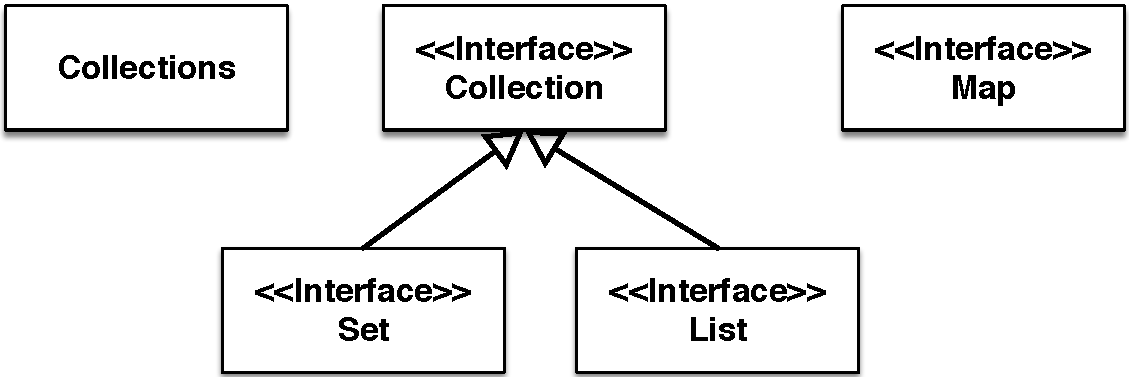
\includegraphics[scale=0.5]{collections_hierarchy_1}
  \end{figure}

  \begin{small}
  \begin{itemize}
  \setlength\itemsep{0.2em}
  \item \codet{Collection}: es la interfaz general que ya fue
    descrita.
    
  \item \codet{Set}: es la interfaz para colecciones \codet{Set}, que
    hereda a \codet{Collection}.
    
  \item \codet{List}: es la interfaz para colecciones \codet{List},
    que hereda a \codet{Collection}.
    
  \item \codet{Collections}: es la clase utilitaria
    \codet{java.util.Collections} con métodos estáticos para
    manipulación de colecciones.

  \item \codet{Map}: es la interfaz para definir estructuras
    \codet{Map}. \textbf{Esta interfaz no hereda desde
      \codet{Collection}}.
    
  \end{itemize}
  \end{small}
  
\end{frame}

\subsection{Interfaz \codet{java.util.Set}}

\begin{frame}[fragile]
  \frametitle{Interfaz \codet{java.util.Set}}

\begin{minted}{java}
public interface Set<E> extends Collection<E>
\end{minted}

  Esta interfaz modela el concepto matemático de \textbf{conjunto}. Es
  una colección de elementos donde no existen duplicados. Dos
  \codet{Set} son iguales solamente si contienen exactamente los
  mismos elementos.

  \begin{block}{Protip}
    A veces queremos eliminar los elementos duplicados de una
    colección, por ejemplo una \codet{List}. Podemos transformar esa
    colección en un \codet{Set}, y luego de vuelta en una
    \codet{List}!
  \end{block}
  
\end{frame}

\begin{frame}[fragile]
  \frametitle{Operaciones sobre \codet{Set}}

  Esta interfaz no agrega nuevas operaciones respecto a las heredadas
  desde \codet{Collection}. Consideremos las variables \codet{Set<E>
    s1, s2}. Es decir dos conjuntos de elementos de tipo \codet{E}. En
  base a las operaciones heredadas desde \codet{Collection} tenemos:

\begin{itemize}

\item \textbf{Unión}: si ejecutamos \codet{s1.addAll(s2)} tendremos
  que \codet{s1} ahora contiene la \textbf{unión} de ambos conjuntos.
 
\item \textbf{Intersección}: si ejecutamos \codet{s1.retainAll(s2)}
  tendremos que \codet{s1} ahora contiene la \textbf{intersección} de
  ambos conjuntos.

\item \textbf{Diferencia}: si ejecutamos \codet{s1.removeAll(s2)}
  tendremos que \codet{s1} ahora contiene la \textbf{diferencia} entre
  \codet{s1} y \codet{s2}.

\item \textbf{Subconjunto}: si ejecutamos \codet{s1.containsAll(s2)}
  sabremos si \codet{s2} es un \textbf{subconjunto} de \codet{s1}.
  
\end{itemize}
  
\end{frame}

\begin{frame}[fragile]
  \frametitle{Ejemplos de \codet{Set}}

  \begin{jsmall}
    class EjemploSet {
      public static void main(String[] args) {
        /** Conjunto de asignaturas de la carrera */        
        Set<Asignatura> s1;

        /** Conjunto de estudiantes de la carrera */        
        Set<Persona> s2;        
      }
    }    
  \end{jsmall}
  
\end{frame}

\subsection{Interfaz \codet{java.util.List}}

\begin{frame}[fragile]
  \frametitle{Interfaz \codet{java.util.List}}

\begin{minted}{java}
public interface List<E> extends Collection<E>
\end{minted}

  Esta interfaz representa una colección secuencial de elementos. Una
  lista puede contener elementos duplicados. Además de las operaciones
  normales de \codet{Collection}, una lista agrega:

  \begin{itemize}

  \item \textbf{Acceso basado en posiciones}: los elementos se pueden
    manipular en base a su posición en la lista.

  \item \textbf{Búsqueda}: al buscar un elemento en la lista se
    obtiene su posición en ella, si es que está contenido.
    
  \end{itemize}  
  
\end{frame}

\begin{frame}
  \frametitle{Interfaz \codet{java.util.List} :: Acceso basado en
    posiciones}

  Los siguientes métodos permiten la manipulación de los elementos de
  la lista según su posición:

  \begin{itemize}
    
  \item \codet{E get(int index)}: retorna el elemento en la
    posición \codet{index}. Si \codet{index} excede el tamaño de la
    lista se arroja una excepción.
    
  \item \codet{E set(int index, E elem)}: inserta el elemento
    \codet{elem} en la posición \codet{index}. Retorna el elemento que
    había antes en esa posición. Arroja excepción si el índice está
    fuera de rango.
    
  \item \codet{boolean add(E e)}: agrega el elemento \codet{e}
    \textbf{al final de la lista}. Si no hay una excepción, siempre
    retorna \codet{true}.

    
  \item \codet{boolean addAll(Collection<? extends E> c)}: agrega
    todos los elementos de \codet{c} al final de la lista. Los agrega
    en el orden en que son devueltos por \codet{c}.
    
  \end{itemize}
  
\end{frame}

\begin{frame}
  \frametitle{Interfaz \codet{java.util.List} :: Búsqueda}

  Los siguientes métodos permiten la búsqueda de elementos en la lista:

  \begin{itemize}
    
  \item \codet{int indexOf(Object o)}: retorna el índice de la primera
    ocurrencia de \codet{o} en la lista, o bien retorna $-1$. Se usa
    el método \codet{equals} para comparar. En otras palabras, el
    índice del elemento ``más a la izquierda o hacia el comienzo'' de
    la lista.
  
  \item \codet{int lastIndexOf(Object o)}: retorna el índice de la
    última ocurrencia de \codet{o} en la lista, o bien retorna
    $-1$. Retorna el elemento ``más a la derecha o hacia el final'' de
    la lista.
    
  \end{itemize}
  
\end{frame}

\begin{frame}[fragile]
  \frametitle{Ejemplos de \codet{List}}

  \begin{jsmall}
    class EjemploList {
      public static void main(String[] args) {
        /** Listado de asignaturas de la carrera */
        List<Asignatura> l1;

        /** Listado de alumnos de la carrera */
        List<Persona>l2;
      }
    }    
  \end{jsmall}
  
\end{frame}


\subsection{Interfaz \codet{java.util.Map}}

\begin{frame}[fragile]
  \frametitle{Interfaz \codet{java.util.Map}}

  Un \codet{Map}---conocido simplemente como ``mapa''---es un objeto
  que mapea o asocia \textbf{llaves} con \textbf{valores}. Se refiere
  al concepto matemático de ``mapeo'', como una función que toma una
  llave como argumento y retorna un valor. Un mapa no puede tener
  llaves repetidas, y cada llave apunta a un solo valor. Los valores
  sí pueden ser repetidos para distintas llaves. También se le conoce
  como \textbf{diccionario}.\\

  Su definición como interfaz es:
  
\begin{minted}{java}
public interface Map<K, V>
\end{minted}

  A diferencia de las interfaces anteriores, \codet{Map} esta
  parametrizado por dos tipos, \codet{K} y \codet{V}:

  \begin{itemize}
    \setlength\itemsep{0.1em}
  \item \codet{K} es el tipo de dato para las llaves    
  \item \codet{V} es el tipo de dato para los valores
  \end{itemize}
  
\end{frame}

\begin{frame}[fragile]
  \frametitle{Ejemplos de \codet{Map}}

  \begin{jsmall}
    class EjemploMap {
      public static void main(String[] args) {
        /** Mapa que asocia enteros con Strings,
        por ejemplo codigos postales con comunas */        
        Map<Integer, String> m1;

        /** Mapa que asocia Strings con Integer,
        por ejemplo nombres de ciudades con su código */
        Map<String, Integer>m2;

        /** Mapa que asocia alumnos con las asignaturas
        que tienen inscritas actualmente */
        Map<Persona, List<Asignatura>>m3;
      }
    }    
  \end{jsmall}
  
\end{frame}

\begin{frame}
  \frametitle{Operaciones sobre \codet{Map}}

  Los siguientes métodos definen las operaciones fundamentales sobre
  \codet{Map}, considerando un mapa \codet{Map<K,V>}:

  \begin{itemize}
    
  \item \codet{V put(K key, V value)}: asocia el valor \codet{value}
    con la llave \codet{key} en el mapa. Retorna el valor anterior
    asociado a esa llave, o bien retorna \codet{null} si no existía
    ninguna asociación.
    
  \item \codet{V get(Object key)}: retorna el valor del mapa que está
    asociado a la llave \codet{key}. Se usa el método \codet{equals}
    para comparar \codet{key} con las llaves existentes. Si el
    elemento no está en el mapa se retorna \codet{null}.
    
  \item \codet{boolean containsKey(Object key)}: retorna \codet{true}
    si el mapa contiene una asociación para la llave \codet{key}; si
    no, retorna \codet{false}.
    
  \item \codet{boolean containsValue(Object value)}: retorna
    \codet{true} si existe una llave que está asociada a un objeto
    igual a \codet{value}. Si no, retorna \codet{false}. Si existe, no
    nos dice qué llaves son...    
    
  \end{itemize}
  
\end{frame}

\begin{frame}
  \frametitle{Mapas como Colecciones}

  Un mapa \codet{Map<K, V} se puede examinar como colecciones gracias
  a los siguientes métodos:

  \begin{itemize}
  \item \codet{Set<K> keySet()}: retorna un conjunto con las llaves
    del mapa.
    
  \item \codet{Collection<V> values()}: retorna una colección con los
    valores del mapa

  \item \codet{Set<Map.Entry<K,V>> entrySet()}: retorna un conjunto
    con las asociaciones del mapa. Las asociaciones son instancias de
    \codet{Map.Entry}; se usan los métodos \codet{getKey} y
    \codet{getValue} para acceder a la llave y valor.
    
  \end{itemize}
  
\end{frame}

\section{Las Implementaciones}

\begin{frame}
  \frametitle{Implementaciones Estándar}

  Una de los mayores beneficios del Java Collections Framework es que
  \textbf{incorpora implementaciones estándar para cada una de las
    colecciones} que hemos descrito anteriormente.

  \begin{figure}
    \centering
    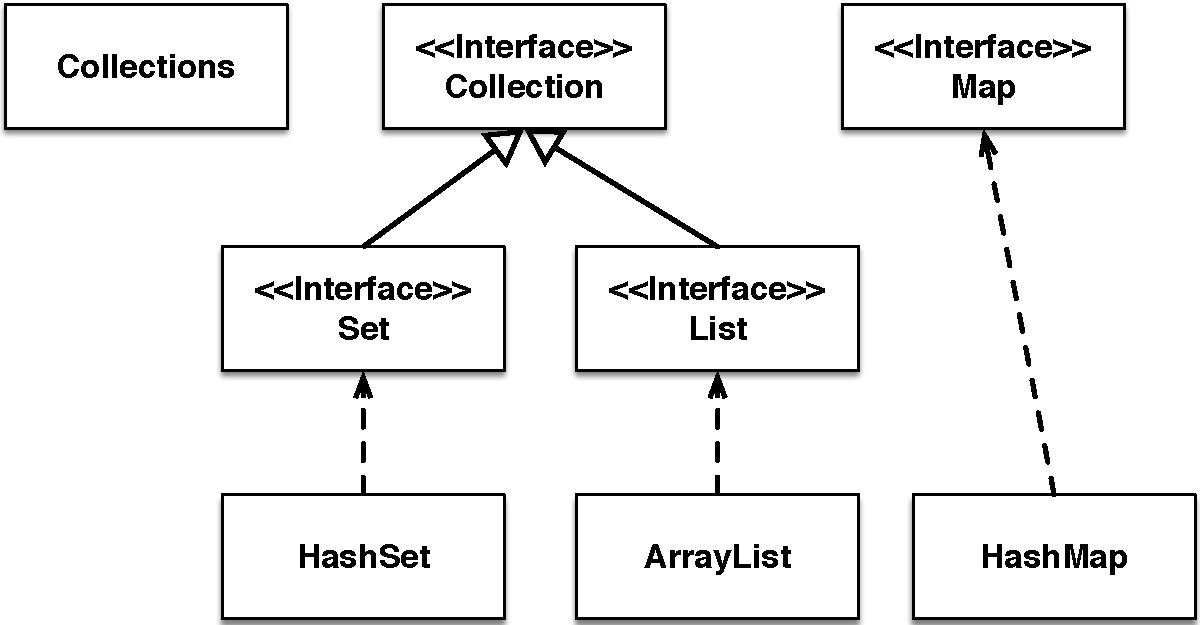
\includegraphics[scale=0.5]{collections_hierarchy_2}
  \end{figure}
  
\end{frame}

\subsection{Implementación de Set}

\begin{frame}[fragile]
  \frametitle{Implementacion de \codet{Set}: \codet{HashSet}}

  \begin{jsmall}
    class EjemploSet {
      public static void main(String[] args) {
        /** Conjunto de asignaturas de la ca,rrera */        
        Set<Asignatura> s1 = new HashSet<Asignatura>();
        Asignatura a1 = new Asignatura("Progra2");
        s1.add(a1);
        s1.add(a1);
        System.out.println(s1.size());

        /** Conjunto de estudiantes de la carrera */        
        Set<Persona> s2 = new HashSet<Persona>();
        s2.add(new Persona(...));
      }
    }    
  \end{jsmall}

  
\end{frame}

\subsection{Implementación de List}

\begin{frame}[fragile]
  \frametitle{Implementacion de \codet{List}: \codet{ArrayList}}

  \begin{jsmall}
    class EjemploList {
      public static void main(String[] args) {
        /** Listado de asignaturas de la carrera */
        List<Asignatura> l1 = new ArrayList<Asignatura>();
        Asignatura a1 = new Asignatura("Progra2");
        l1.add(a1);
        l1.add(a1);
        System.out.println(l1.size());
        
        /** Listado de alumnos de la carrera */
        List<Persona>l2 = new ArrayList<Asignatura>();
        l2.add(new Persona(...));
      }
    }    
  \end{jsmall}
  
\end{frame}

\subsection{Implementación de Map}

\begin{frame}[fragile]
  \frametitle{Implementacion de \codet{Map}: \codet{HashMap}}

  \begin{jsmall}
    class EjemploMap {
      public static void main(String[] args) {
        Map<Integer, String> m1 = new HashMap<Integer, String>();
        Map<String, Integer>m2 = new HashMap<String, Integer>();

        /** Mapa que asocia alumnos con las
        asignaturas que tienen inscritas actualmente */
        Map<Persona, List<Asignatura>>m3 =
        new HashMap<Persona, List<Asignatura>>();
        
        Persona p1 = new Persona("Juanito");
        Asignatura a1 = new Asignatura("Progra2");
        
        m3.put(p1, new ArrayList<Asignatura>(a1));

        Asignatura a2 = new Asignatura("Calculo");
        m3.get(p1).add(a2);        
      }
    }    
  \end{jsmall}  
\end{frame}

\subsection{Interfaces vs Clases Concretas}

\begin{frame}
  \frametitle{¿Interface o Clase Concreta?}

  \begin{alertblock}{}
    Siempre es mejor \textbf{programar para satisfacer interfaces
      generales} más que para clases o implementaciones
    específicas. \textbf{Así podremos aprovechar el polimorfismo
      basado en interfaces!}
  \end{alertblock}
  
\end{frame}

\begin{frame}[fragile]
  \frametitle{¿Interface o Clase Concreta? ---- Variables}

  \begin{jsmall}
    public static void main(String[] args) {
      Set<Persona> alumnos = new HashSet<Persona>();
      // Mantiene abierta la opcion sobre cual implementación
      // ... de Set utilizar, promueve polimorfismo
      
    }
  \end{jsmall}

  \begin{jsmall}
    public static void main(String[] args) {
      HashSet<Persona> alumnos = new HashSet<Persona>();
      // Deja cerrada la opción sobre la implementación
      // ... no permite polimorfismo, puede ser dificil después
      // ... cambiar por otra implementación
    }
  \end{jsmall}
  
\end{frame}

\begin{frame}[fragile]
  \frametitle{¿Interface o Clase Concreta? --- Métodos}

  \begin{jsmall}
    public class Ejemplo {

      public Double promedioNotas(List<Double> notas) {
        // Implementacion usando interfaz List
        // ... Se puede invocar pasando cualquier objeto que implemente List
      }
    }
  \end{jsmall}
  \begin{jsmall}       
    public class Ejemplo {

      public Double promedioNotas(ArrayList<Double> notas) {
        // Implementacion usando ArrayList
        // ... Solo se puede invocar para objetos de tipo ArrayList
      }
    }    
  \end{jsmall}

\end{frame}

\begin{frame}
  \frametitle{Preguntas}
  \hspace{4cm}\huge{Preguntas?}  
\end{frame}

\end{document}